% Parte 07 — Stewart, Precálculo 7.ª ed., §2.7 "Combinación de funciones" (pp. 210–218)
% Ejercicios elegidos (número + página del libro):
%   9  (p. 216) — f+g, f-g, fg, f/g y sus dominios (polinomios)
%   13 (p. 216) — combinación con radicales y dominios
%   15 (p. 216) — combinación con funciones racionales
%   17 (p. 216) — dominio de una suma de radicales
%   20 (p. 216) — dominio de un cociente con radical
%   29 (p. 216) — evaluar (f o g)(-2) y (g o f)(-2)
%   31 (p. 216) — (f o g)(x) y (g o f)(x)
%   35 (p. 217) — (g o f)(4) leyendo la gráfica  [figura fig_p07_35.png]
%   45 (p. 217) — (f o f)(5) usando una tabla
%   49 (p. 217) — f o g, g o f, f o f, g o g y sus dominios
%   55 (p. 217) — lo mismo, con dominios finos (racional)
%   59 (p. 217) — composición triple f o g o h
%   63 (p. 217) — expresar F en la forma f o g
%   69 (p. 217) — expresar F en la forma f o g o h
%   77 (p. 218) — aplicación: área de una onda circular
% Figuras extraídas: fig_p07_35.png (gráfica de f y g, p. 217).

\documentclass[11pt]{article}
\usepackage[utf8]{inputenc}
\usepackage[spanish]{babel}
\usepackage[margin=2.3cm]{geometry}
\usepackage{amsmath,amssymb}
\usepackage{enumitem}
\usepackage{tcolorbox}
\tcbuselibrary{skins,breakable}
\usepackage{pgfplots}
\pgfplotsset{compat=1.18}
\usepackage{tikz}
\usepackage{graphicx}
\usepackage{array}
\usepackage[hidelinks]{hyperref}

% Notación española opcional (descomenta si quieres \sen en lugar de \sin)
% \DeclareMathOperator{\sen}{sen}
% \DeclareMathOperator{\tg}{tg}
% \DeclareMathOperator{\ctg}{ctg}

\newtcolorbox{sol}{colback=blue!5,colframe=blue!50!black,title=Solución paso a paso,breakable}
\newtcolorbox{teo}{colback=orange!8,colframe=orange!70!black,title=Teoría,breakable}
\newtcolorbox{nota}{colback=green!5,colframe=green!50!black,title=Idea clave,breakable}
\newtcolorbox{tip}{colback=yellow!10,colframe=yellow!60!black,title=Consejo,breakable}
\newtcolorbox{resp}{colback=red!5,colframe=red!50!black,title=Respuesta,breakable}
\newtcolorbox{reg}{colback=red!5,colframe=red!60!black,title=Regla,breakable}
\newtcolorbox{paso}[1]{colback=gray!5,colframe=gray!50!black,title={#1},breakable}

\graphicspath{{../images/}{images/}}
\newcommand{\sen}{\operatorname{sen}}

% babel spanish activa < y > y rompe TikZ/pgfplots (->, >=stealth)
\AtBeginDocument{\shorthandoff{<>}}

\begin{document}

\section*{Parte 07 — Combinación de funciones (Stewart §2.7, pp. 210–218)}

\begin{teo}
\textbf{Método de la sección.}
\begin{enumerate}[leftmargin=*]
\item \textbf{Álgebra de funciones.} Si $f$ tiene dominio $A$ y $g$ tiene dominio $B$:
\[
(f+g)(x)=f(x)+g(x),\quad (f-g)(x)=f(x)-g(x),\quad (fg)(x)=f(x)g(x),
\]
las tres con dominio $A\cap B$, porque hay que poder evaluar \emph{ambas} funciones.
\item \textbf{Cociente.} $\left(\dfrac{f}{g}\right)(x)=\dfrac{f(x)}{g(x)}$ con dominio $\{x\in A\cap B \mid g(x)\neq 0\}$: además de evaluar las dos, no se divide entre $0$.
\item \textbf{Composición.} $(f\circ g)(x)=f(g(x))$: primero actúa $g$, después $f$. El orden importa; en general $f\circ g\neq g\circ f$.
\item \textbf{Dominio de la composición.} $\operatorname{dom}(f\circ g)=\{x\in \operatorname{dom} g \mid g(x)\in \operatorname{dom} f\}$. Se imponen las dos condiciones \emph{antes} de simplificar: la fórmula simplificada puede tener sentido en puntos que la composición no admite.
\item \textbf{Evaluación en un punto.} Para $(f\circ g)(a)$ se calcula $g(a)$ y ese número se mete en $f$. Con gráficas o tablas es idéntico: se lee $g(a)$ y luego se lee $f$ en ese valor.
\item \textbf{Descomposición.} Para escribir $F$ como $f\circ g$ se toma como $g$ lo que está \emph{dentro} (el bloque que se repite o el argumento de la operación externa) y como $f$ la operación que se aplica al final.
\end{enumerate}
\end{teo}

\begin{tip}
Restricciones que se usan todo el tiempo en esta sección:
\begin{itemize}[leftmargin=*]
\item Radicando de índice par: $\sqrt{u}$ exige $u\ge 0$.
\item Denominador: $\dfrac{1}{u}$ exige $u\neq 0$.
\item $\sqrt{a}\,\sqrt{b}=\sqrt{ab}$ y $\dfrac{\sqrt{a}}{\sqrt{b}}=\sqrt{\dfrac{a}{b}}$ (válidas con $a\ge 0$, $b>0$).
\item $25-x^2\ge 0 \iff -5\le x\le 5$ (la parábola $25-x^2$ es $\ge 0$ entre sus ceros $\pm 5$).
\end{itemize}
\end{tip}

% ============================================================
\subsection*{Ejercicio 1 — Combinación de dos polinomios (libro 9, p. 216)}

\begin{quote}
\textbf{7--16 $\blacksquare$ Combinación de funciones} \quad Encuentre $f+g$, $f-g$, $fg$ y $f/g$ y sus dominios.

\textbf{9.} $f(x)=x^2+x, \quad g(x)=x^2$
\end{quote}

\begin{paso}{Paso 1 --- Dominios de $f$ y de $g$}
\textbf{Qué hago:} identifico $A=\operatorname{dom} f$ y $B=\operatorname{dom} g$.

\textbf{¿De dónde sale?} Del enunciado: $f(x)=x^2+x$ y $g(x)=x^2$ son polinomios, sin denominadores ni radicales.

\textbf{¿Por qué?} Un polinomio está definido para todo real, así que $A=B=\mathbb{R}$ y $A\cap B=\mathbb{R}$.
\end{paso}

\begin{paso}{Paso 2 --- Suma, diferencia y producto}
\textbf{Qué hago:} aplico las definiciones $(f\pm g)(x)=f(x)\pm g(x)$ y $(fg)(x)=f(x)g(x)$, y reduzco términos semejantes.

\textbf{¿De dónde sale?} De las fórmulas del álgebra de funciones con $f(x)=x^2+x$, $g(x)=x^2$.

\textbf{¿Por qué?} Los tres tienen dominio $A\cap B=\mathbb{R}$.
\[
(f+g)(x)=(x^2+x)+x^2=2x^2+x,\qquad
(f-g)(x)=(x^2+x)-x^2=x,
\]
\[
(fg)(x)=(x^2+x)x^2=x^4+x^3 .
\]
\end{paso}

\begin{paso}{Paso 3 --- Cociente y su dominio}
\textbf{Qué hago:} formo $f/g$ y le quito los ceros de $g$.

\textbf{¿De dónde sale?} $g(x)=x^2=0$ solo en $x=0$.

\textbf{¿Por qué?} El dominio de $f/g$ es $\{x\in A\cap B\mid g(x)\neq 0\}$, porque no se divide entre $0$.
\[
\left(\frac{f}{g}\right)(x)=\frac{x^2+x}{x^2}=\frac{x(x+1)}{x^2}=\frac{x+1}{x},\qquad x\neq 0 .
\]
\end{paso}

\begin{resp}
$(f+g)(x)=2x^2+x$, $(f-g)(x)=x$, $(fg)(x)=x^4+x^3$, todas con dominio $\mathbb{R}$;\\
$\left(\dfrac{f}{g}\right)(x)=\dfrac{x+1}{x}$ con dominio $\{x\mid x\neq 0\}=(-\infty,0)\cup(0,\infty)$.
\end{resp}

% ============================================================
\subsection*{Ejercicio 2 — Combinación con radicales (libro 13, p. 216)}

\begin{quote}
\textbf{13.} $f(x)=\sqrt{25-x^2}, \quad g(x)=\sqrt{x+3}$
\end{quote}

\begin{paso}{Paso 1 --- Dominio de cada función}
\textbf{Qué hago:} exijo radicando $\ge 0$ en cada una.

\textbf{¿De dónde sale?} De los radicandos $25-x^2$ y $x+3$ del enunciado.

\textbf{¿Por qué?} La raíz de índice par solo está definida para argumentos no negativos en los reales.
\[
25-x^2\ge 0 \iff -5\le x\le 5 \;\Rightarrow\; A=[-5,5];\qquad
x+3\ge 0 \iff x\ge -3 \;\Rightarrow\; B=[-3,\infty).
\]
\end{paso}

\begin{paso}{Paso 2 --- Intersección de dominios}
\textbf{Qué hago:} corto $A$ con $B$.

\textbf{¿De dónde sale?} De $A=[-5,5]$ y $B=[-3,\infty)$ del paso 1.

\textbf{¿Por qué?} Suma, diferencia y producto tienen dominio $A\cap B$, pues requieren evaluar las dos funciones.
\[
A\cap B=[-3,5].
\]
\end{paso}

\begin{paso}{Paso 3 --- Las cuatro combinaciones}
\textbf{Qué hago:} escribo $f\pm g$, $fg$ y $f/g$, usando $\sqrt{a}\sqrt{b}=\sqrt{ab}$ y $\sqrt{a}/\sqrt{b}=\sqrt{a/b}$ en las dos últimas.

\textbf{¿De dónde sale?} De las definiciones del álgebra de funciones con las $f$ y $g$ dadas.

\textbf{¿Por qué?} Ambas raíces son no negativas en $[-3,5]$, que es donde valen esas identidades de radicales.
\[
(f+g)(x)=\sqrt{25-x^2}+\sqrt{x+3},\qquad (f-g)(x)=\sqrt{25-x^2}-\sqrt{x+3},
\]
\[
(fg)(x)=\sqrt{(25-x^2)(x+3)},\qquad \left(\frac{f}{g}\right)(x)=\sqrt{\frac{25-x^2}{x+3}} .
\]
\end{paso}

\begin{paso}{Paso 4 --- Ajuste del dominio del cociente}
\textbf{Qué hago:} elimino de $[-3,5]$ los puntos donde $g$ se anula.

\textbf{¿De dónde sale?} $g(x)=\sqrt{x+3}=0$ exactamente en $x=-3$, que es el extremo izquierdo de $A\cap B$.

\textbf{¿Por qué?} El dominio de $f/g$ excluye los ceros de $g$; el intervalo queda abierto en $-3$.
\[
\operatorname{dom}\left(\frac{f}{g}\right)=(-3,5].
\]
\end{paso}

\begin{resp}
$(f+g)(x)=\sqrt{25-x^2}+\sqrt{x+3}$, $(f-g)(x)=\sqrt{25-x^2}-\sqrt{x+3}$, $(fg)(x)=\sqrt{(25-x^2)(x+3)}$, las tres con dominio $[-3,5]$;\\
$\left(\dfrac{f}{g}\right)(x)=\sqrt{\dfrac{25-x^2}{x+3}}$ con dominio $(-3,5]$.
\end{resp}

% ============================================================
\subsection*{Ejercicio 3 — Combinación de funciones racionales (libro 15, p. 216)}

\begin{quote}
\textbf{15.} $f(x)=\dfrac{2}{x}, \quad g(x)=\dfrac{4}{x+4}$
\end{quote}

\begin{paso}{Paso 1 --- Dominios y su intersección}
\textbf{Qué hago:} exijo denominador distinto de cero en cada función.

\textbf{¿De dónde sale?} De los denominadores $x$ y $x+4$ del enunciado.

\textbf{¿Por qué?} La división entre $0$ no está definida, así que $A=\{x\mid x\neq 0\}$, $B=\{x\mid x\neq -4\}$ y $A\cap B=\{x\mid x\neq 0,\ x\neq -4\}$.
\end{paso}

\begin{paso}{Paso 2 --- Suma y diferencia con denominador común}
\textbf{Qué hago:} sumo y resto las fracciones usando el común denominador $x(x+4)$.

\textbf{¿De dónde sale?} De $f(x)=2/x$ y $g(x)=4/(x+4)$: $\dfrac{2}{x}=\dfrac{2(x+4)}{x(x+4)}$ y $\dfrac{4}{x+4}=\dfrac{4x}{x(x+4)}$.

\textbf{¿Por qué?} $(f\pm g)(x)=f(x)\pm g(x)$, y ambas tienen dominio $A\cap B$.
\[
(f+g)(x)=\frac{2(x+4)+4x}{x(x+4)}=\frac{6x+8}{x(x+4)},\qquad
(f-g)(x)=\frac{2(x+4)-4x}{x(x+4)}=\frac{8-2x}{x(x+4)} .
\]
\end{paso}

\begin{paso}{Paso 3 --- Producto y cociente}
\textbf{Qué hago:} multiplico y luego divido (multiplicando por el recíproco).

\textbf{¿De dónde sale?} $\dfrac{2}{x}\cdot\dfrac{4}{x+4}$ y $\dfrac{2}{x}\div\dfrac{4}{x+4}=\dfrac{2}{x}\cdot\dfrac{x+4}{4}$.

\textbf{¿Por qué?} Son las definiciones de $(fg)$ y $(f/g)$.
\[
(fg)(x)=\frac{8}{x(x+4)},\qquad \left(\frac{f}{g}\right)(x)=\frac{2(x+4)}{4x}=\frac{x+4}{2x} .
\]
\end{paso}

\begin{paso}{Paso 4 --- Dominios de producto y cociente}
\textbf{Qué hago:} reviso si $g$ tiene ceros y arrastro $A\cap B$.

\textbf{¿De dónde sale?} $g(x)=\dfrac{4}{x+4}$ nunca vale $0$, porque un cociente es $0$ solo si su numerador lo es y aquí el numerador es $4$.

\textbf{¿Por qué?} El dominio de $f/g$ es $\{x\in A\cap B\mid g(x)\neq 0\}$: al no haber ceros, queda $A\cap B$ tal cual, aunque la forma simplificada $\dfrac{x+4}{2x}$ parezca aceptar $x=-4$.
\end{paso}

\begin{resp}
$(f+g)(x)=\dfrac{6x+8}{x(x+4)}$, \; $(f-g)(x)=\dfrac{8-2x}{x(x+4)}$, \; $(fg)(x)=\dfrac{8}{x(x+4)}$, \; $\left(\dfrac{f}{g}\right)(x)=\dfrac{x+4}{2x}$.\\[2pt]
Las cuatro tienen dominio $\{x\mid x\neq -4 \text{ y } x\neq 0\}=(-\infty,-4)\cup(-4,0)\cup(0,\infty)$.
\end{resp}

% ============================================================
\subsection*{Ejercicio 4 — Dominio de una suma de radicales (libro 17, p. 216)}

\begin{quote}
\textbf{17--20 $\blacksquare$ Dominio} \quad Encuentre el dominio de la función.

\textbf{17.} $f(x)=\sqrt{x}+\sqrt{3-x}$
\end{quote}

\begin{paso}{Paso 1 --- Una restricción por cada raíz}
\textbf{Qué hago:} exijo que los dos radicandos sean $\ge 0$ a la vez.

\textbf{¿De dónde sale?} Del enunciado: los radicandos son $x$ y $3-x$.

\textbf{¿Por qué?} $f$ es la suma de dos funciones, y el dominio de una suma es la intersección de los dominios.
\[
x\ge 0 \quad\text{y}\quad 3-x\ge 0 \iff x\le 3 .
\]
\end{paso}

\begin{paso}{Paso 2 --- Intersección}
\textbf{Qué hago:} corto $[0,\infty)$ con $(-\infty,3]$.

\textbf{¿De dónde sale?} De las dos desigualdades del paso 1.

\textbf{¿Por qué?} Ambas condiciones deben cumplirse simultáneamente para poder sumar.
\end{paso}

\begin{resp}
$\operatorname{dom} f=[0,3]$.
\end{resp}

% ============================================================
\subsection*{Ejercicio 5 — Dominio de un cociente con radical (libro 20, p. 216)}

\begin{quote}
\textbf{20.} $k(x)=\dfrac{\sqrt{x+3}}{x-1}$
\end{quote}

\begin{paso}{Paso 1 --- Restricción del radicando}
\textbf{Qué hago:} exijo $x+3\ge 0$.

\textbf{¿De dónde sale?} Del numerador $\sqrt{x+3}$.

\textbf{¿Por qué?} Raíz de índice par: solo está definida para argumento no negativo.
\[
x+3\ge 0 \iff x\ge -3 .
\]
\end{paso}

\begin{paso}{Paso 2 --- Restricción del denominador}
\textbf{Qué hago:} exijo $x-1\neq 0$.

\textbf{¿De dónde sale?} Del denominador $x-1$; se anula en $x=1$.

\textbf{¿Por qué?} $k$ es el cociente de $\sqrt{x+3}$ entre $x-1$, y el dominio del cociente excluye los ceros del divisor.
\end{paso}

\begin{paso}{Paso 3 --- Combino ambas}
\textbf{Qué hago:} tomo $x\ge -3$ y le quito $x=1$, que cae dentro de ese conjunto.

\textbf{¿De dónde sale?} De los pasos 1 y 2.

\textbf{¿Por qué?} Las dos condiciones se exigen a la vez.
\end{paso}

\begin{resp}
$\operatorname{dom} k=[-3,1)\cup(1,\infty)$.
\end{resp}

% ============================================================
\subsection*{Ejercicio 6 — Evaluar composiciones en un punto (libro 29, p. 216)}

\begin{quote}
\textbf{27--32 $\blacksquare$ Evaluación de funciones compuestas} \quad Use $f(x)=2x-3$ y $g(x)=4-x^2$ para evaluar la expresión.

\textbf{29.} \; \textbf{\emph{a}}) $(f\circ g)(-2)$ \hfill \textbf{\emph{b}}) $(g\circ f)(-2)$
\end{quote}

\begin{paso}{Paso 1 --- (a) Evalúo primero la función interior}
\textbf{Qué hago:} calculo $g(-2)$ y meto el resultado en $f$.

\textbf{¿De dónde sale?} De $g(x)=4-x^2$ con $x=-2$, y luego de $f(x)=2x-3$.

\textbf{¿Por qué?} Por definición $(f\circ g)(-2)=f(g(-2))$: en una composición actúa primero la función de adentro.
\[
g(-2)=4-(-2)^2=4-4=0,\qquad (f\circ g)(-2)=f(0)=2(0)-3=-3 .
\]
\end{paso}

\begin{paso}{Paso 2 --- (b) Invierto el orden}
\textbf{Qué hago:} calculo $f(-2)$ y meto el resultado en $g$.

\textbf{¿De dónde sale?} De $f(x)=2x-3$ con $x=-2$, y luego de $g(x)=4-x^2$.

\textbf{¿Por qué?} $(g\circ f)(-2)=g(f(-2))$; el resultado distinto al de (a) confirma que la composición no es conmutativa.
\[
f(-2)=2(-2)-3=-7,\qquad (g\circ f)(-2)=g(-7)=4-(-7)^2=4-49=-45 .
\]
\end{paso}

\begin{resp}
\textbf{a)} $(f\circ g)(-2)=-3$. \qquad \textbf{b)} $(g\circ f)(-2)=-45$.
\end{resp}

% ============================================================
\subsection*{Ejercicio 7 — Composiciones como fórmula (libro 31, p. 216)}

\begin{quote}
\textbf{31.} \; \textbf{\emph{a}}) $(f\circ g)(x)$ \hfill \textbf{\emph{b}}) $(g\circ f)(x)$

\noindent{\small(con $f(x)=2x-3$ y $g(x)=4-x^2$, del encabezado 27--32)}
\end{quote}

\begin{paso}{Paso 1 --- (a) Sustituyo $g(x)$ dentro de $f$}
\textbf{Qué hago:} reemplazo la variable de $f(x)=2x-3$ por la expresión completa $4-x^2$ y desarrollo.

\textbf{¿De dónde sale?} De la definición $(f\circ g)(x)=f(g(x))$ con $g(x)=4-x^2$.

\textbf{¿Por qué?} $f$ multiplica por $2$ y resta $3$ a lo que reciba, sea un número o una expresión.
\[
(f\circ g)(x)=2(4-x^2)-3=8-2x^2-3=5-2x^2 .
\]
\end{paso}

\begin{paso}{Paso 2 --- (b) Sustituyo $f(x)$ dentro de $g$}
\textbf{Qué hago:} reemplazo la variable de $g(x)=4-x^2$ por $2x-3$ y desarrollo el binomio al cuadrado.

\textbf{¿De dónde sale?} De $(g\circ f)(x)=g(f(x))$ y de $(2x-3)^2=4x^2-12x+9$ (cuadrado de un binomio).

\textbf{¿Por qué?} El signo menos afecta a todo el cuadrado, no solo al primer término.
\[
(g\circ f)(x)=4-(2x-3)^2=4-(4x^2-12x+9)=-4x^2+12x-5 .
\]
\end{paso}

\begin{resp}
\textbf{a)} $(f\circ g)(x)=5-2x^2$. \qquad \textbf{b)} $(g\circ f)(x)=-4x^2+12x-5$.\\
Ambas con dominio $\mathbb{R}$, pues $f$ y $g$ son polinomios.
\end{resp}

% ============================================================
\subsection*{Ejercicio 8 — Composición leída en una gráfica (libro 35, p. 217)}

\begin{quote}
\textbf{33--38 $\blacksquare$ Composición usando una gráfica} \quad Use las gráficas dadas de $f$ y $g$ para evaluar la expresión.

\begin{center}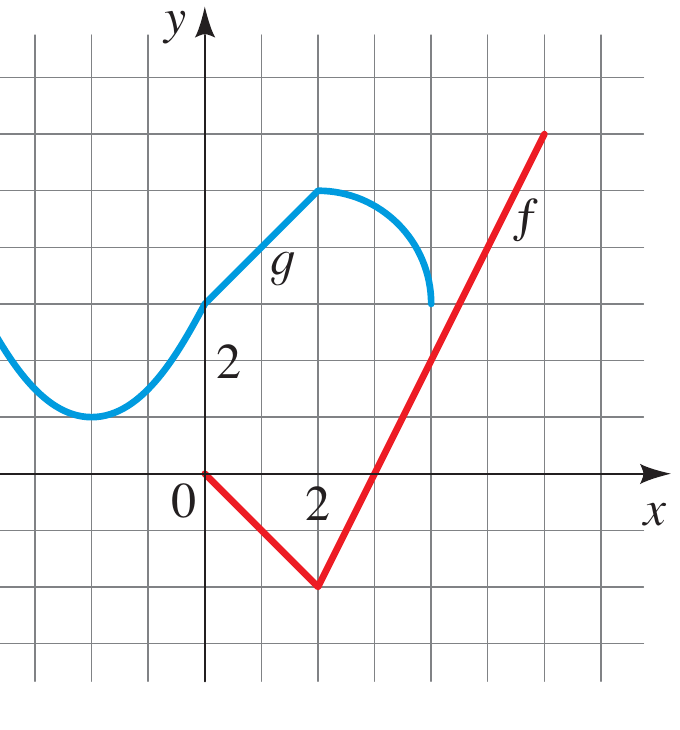
\includegraphics[width=0.5\textwidth]{fig_p07_35.png}\end{center}

\textbf{35.} $(g\circ f)(4)$
\end{quote}

\begin{paso}{Paso 1 --- Leo $f(4)$ en la gráfica roja}
\textbf{Qué hago:} localizo $x=4$ y subo hasta la curva roja, etiquetada $f$.

\textbf{¿De dónde sale?} De la gráfica: $f$ es la ``V'' con vértice en $(2,-2)$; en $x=4$ la rama derecha está dos unidades sobre el eje $x$.

\textbf{¿Por qué?} La gráfica de $f$ es el conjunto de puntos $(x,f(x))$, así que la altura en $x=4$ \emph{es} $f(4)$.
\[
f(4)=2 .
\]
\end{paso}

\begin{paso}{Paso 2 --- Leo $g$ en ese resultado}
\textbf{Qué hago:} evalúo $g$ en $2$, es decir, localizo $x=2$ y subo hasta la curva azul $g$.

\textbf{¿De dónde sale?} Del paso 1: $f(4)=2$, y $(g\circ f)(4)=g(f(4))=g(2)$.

\textbf{¿Por qué?} En $x=2$ la curva azul alcanza su punto más alto, cinco unidades sobre el eje $x$.
\[
g(2)=5 .
\]
\end{paso}

\begin{resp}
$(g\circ f)(4)=5$.
\end{resp}

% ============================================================
\subsection*{Ejercicio 9 — Composición leída en una tabla (libro 45, p. 217)}

\begin{quote}
\textbf{39--46 $\blacksquare$ Composición usando una tabla} \quad Use la tabla para evaluar la expresión.

\begin{center}
\begin{tabular}{|c|c|c|c|c|c|c|}
\hline
$x$ & 1 & 2 & 3 & 4 & 5 & 6 \\ \hline
$f(x)$ & 2 & 3 & 5 & 1 & 6 & 3 \\ \hline
$g(x)$ & 3 & 5 & 6 & 2 & 1 & 4 \\ \hline
\end{tabular}
\end{center}

\textbf{45.} $(f\circ f)(5)$
\end{quote}

\begin{paso}{Paso 1 --- Aplico $f$ una primera vez}
\textbf{Qué hago:} leo en la fila $f(x)$ el valor correspondiente a $x=5$.

\textbf{¿De dónde sale?} De la columna $x=5$ de la tabla.

\textbf{¿Por qué?} $(f\circ f)(5)=f(f(5))$: la función interior se evalúa primero.
\[
f(5)=6 .
\]
\end{paso}

\begin{paso}{Paso 2 --- Aplico $f$ otra vez, ahora en $6$}
\textbf{Qué hago:} leo $f(6)$ en la misma fila.

\textbf{¿De dónde sale?} Del paso 1, que entrega $6$ como nueva entrada, y de la columna $x=6$.

\textbf{¿Por qué?} La salida de la primera aplicación es la entrada de la segunda, por definición de composición.
\[
f(6)=3 .
\]
\end{paso}

\begin{resp}
$(f\circ f)(5)=3$.
\end{resp}

% ============================================================
\subsection*{Ejercicio 10 — Las cuatro composiciones (libro 49, p. 217)}

\begin{quote}
\textbf{47--58 $\blacksquare$ Composición de funciones} \quad Encuentre $f\circ g$, $g\circ f$, $f\circ f$ y $g\circ g$ y sus dominios.

\textbf{49.} $f(x)=x^2, \quad g(x)=x+1$
\end{quote}

\begin{paso}{Paso 1 --- $f\circ g$ y $g\circ f$}
\textbf{Qué hago:} sustituyo una función dentro de la otra en los dos órdenes.

\textbf{¿De dónde sale?} De $f(x)=x^2$ y $g(x)=x+1$.

\textbf{¿Por qué?} $f$ eleva al cuadrado lo que recibe y $g$ le suma $1$; el orden cambia el resultado.
\[
(f\circ g)(x)=f(x+1)=(x+1)^2,\qquad (g\circ f)(x)=g(x^2)=x^2+1 .
\]
\end{paso}

\begin{paso}{Paso 2 --- $f\circ f$ y $g\circ g$}
\textbf{Qué hago:} compongo cada función consigo misma.

\textbf{¿De dónde sale?} De las mismas fórmulas, usando $(x^2)^2=x^4$ (ley de exponentes) y $(x+1)+1=x+2$.

\textbf{¿Por qué?} La definición de composición no exige funciones distintas.
\[
(f\circ f)(x)=f(x^2)=(x^2)^2=x^4,\qquad (g\circ g)(x)=g(x+1)=(x+1)+1=x+2 .
\]
\end{paso}

\begin{paso}{Paso 3 --- Dominios}
\textbf{Qué hago:} aplico $\operatorname{dom}(f\circ g)=\{x\in\operatorname{dom} g \mid g(x)\in\operatorname{dom} f\}$ a los cuatro casos.

\textbf{¿De dónde sale?} $f$ y $g$ son polinomios, con dominio $\mathbb{R}$ cada uno.

\textbf{¿Por qué?} Ninguna condición se viola: toda $x$ real está en el dominio de la interior y toda salida real está en el dominio de la exterior.
\end{paso}

\begin{resp}
$(f\circ g)(x)=(x+1)^2$, $(g\circ f)(x)=x^2+1$, $(f\circ f)(x)=x^4$, $(g\circ g)(x)=x+2$; las cuatro con dominio $\mathbb{R}$.
\end{resp}

% ============================================================
\subsection*{Ejercicio 11 — Composiciones con dominios restringidos (libro 55, p. 217)}

\begin{quote}
\textbf{55.} $f(x)=\dfrac{x}{x+1}, \quad g(x)=2x-1$
\end{quote}

\begin{paso}{Paso 1 --- Dominios de partida}
\textbf{Qué hago:} anoto $\operatorname{dom} f$ y $\operatorname{dom} g$.

\textbf{¿De dónde sale?} $f$ tiene denominador $x+1$, que se anula en $x=-1$; $g$ es lineal.

\textbf{¿Por qué?} No se divide entre $0$: $\operatorname{dom} f=\{x\mid x\neq -1\}$ y $\operatorname{dom} g=\mathbb{R}$.
\end{paso}

\begin{paso}{Paso 2 --- $f\circ g$ y su dominio}
\textbf{Qué hago:} sustituyo $2x-1$ en $f$ y exijo que esa entrada esté en $\operatorname{dom} f$.

\textbf{¿De dónde sale?} $f(2x-1)=\dfrac{2x-1}{(2x-1)+1}=\dfrac{2x-1}{2x}$; la condición es $2x-1\neq -1$, o sea $x\neq 0$.

\textbf{¿Por qué?} $\operatorname{dom}(f\circ g)=\{x\in\operatorname{dom} g\mid g(x)\in\operatorname{dom} f\}$; aquí la restricción coincide con el denominador $2x$ que aparece al simplificar.
\[
(f\circ g)(x)=\frac{2x-1}{2x},\qquad \operatorname{dom}=\{x\mid x\neq 0\}.
\]
\end{paso}

\begin{paso}{Paso 3 --- $g\circ f$ y su dominio}
\textbf{Qué hago:} sustituyo $f(x)$ en $g$ y junto en una sola fracción.

\textbf{¿De dónde sale?} $g\!\left(\dfrac{x}{x+1}\right)=2\cdot\dfrac{x}{x+1}-1=\dfrac{2x-(x+1)}{x+1}=\dfrac{x-1}{x+1}$.

\textbf{¿Por qué?} La única restricción es $x\in\operatorname{dom} f$, es decir $x\neq -1$, porque $\operatorname{dom} g=\mathbb{R}$ acepta cualquier salida de $f$.
\[
(g\circ f)(x)=\frac{x-1}{x+1},\qquad \operatorname{dom}=\{x\mid x\neq -1\}.
\]
\end{paso}

\begin{paso}{Paso 4 --- $f\circ f$ y su dominio}
\textbf{Qué hago:} sustituyo $f$ en sí misma y simplifico la fracción compuesta.

\textbf{¿De dónde sale?} $\dfrac{\frac{x}{x+1}}{\frac{x}{x+1}+1}=\dfrac{\frac{x}{x+1}}{\frac{2x+1}{x+1}}=\dfrac{x}{2x+1}$.

\textbf{¿Por qué?} Hay dos condiciones: $x\neq -1$ (para poder calcular $f(x)$) y $f(x)\neq -1$, que da $\dfrac{x}{x+1}=-1\Rightarrow x=-x-1\Rightarrow x=-\tfrac12$; esta última se pierde si uno solo mira la fórmula simplificada.
\[
(f\circ f)(x)=\frac{x}{2x+1},\qquad \operatorname{dom}=\left\{x\ \middle|\ x\neq -1,\ x\neq -\tfrac12\right\}.
\]
\end{paso}

\begin{paso}{Paso 5 --- $g\circ g$ y su dominio}
\textbf{Qué hago:} sustituyo $g$ en sí misma.

\textbf{¿De dónde sale?} $g(2x-1)=2(2x-1)-1=4x-3$.

\textbf{¿Por qué?} $\operatorname{dom} g=\mathbb{R}$ y toda salida real vuelve a estar en $\operatorname{dom} g$, así que no hay restricciones.
\end{paso}

\begin{resp}
$(f\circ g)(x)=\dfrac{2x-1}{2x}$, dominio $\{x\mid x\neq 0\}$;\quad
$(g\circ f)(x)=\dfrac{x-1}{x+1}$, dominio $\{x\mid x\neq -1\}$;\\[2pt]
$(f\circ f)(x)=\dfrac{x}{2x+1}$, dominio $\left\{x\mid x\neq -1,\ x\neq -\tfrac12\right\}$;\quad
$(g\circ g)(x)=4x-3$, dominio $\mathbb{R}$.
\end{resp}

% ============================================================
\subsection*{Ejercicio 12 — Composición de tres funciones (libro 59, p. 217)}

\begin{quote}
\textbf{59--62 $\blacksquare$ Composición de tres funciones} \quad Encuentre $f\circ g\circ h$.

\textbf{59.} $f(x)=x-1, \quad g(x)=\sqrt{x}, \quad h(x)=x-1$
\end{quote}

\begin{paso}{Paso 1 --- Aplico $h$ y luego $g$}
\textbf{Qué hago:} calculo $g(h(x))$ trabajando de adentro hacia afuera.

\textbf{¿De dónde sale?} $h(x)=x-1$ y $g$ toma raíz cuadrada de lo que recibe.

\textbf{¿Por qué?} $(f\circ g\circ h)(x)=f(g(h(x)))$: la composición se asocia de derecha a izquierda.
\[
g(h(x))=\sqrt{x-1}.
\]
\end{paso}

\begin{paso}{Paso 2 --- Aplico $f$ al resultado}
\textbf{Qué hago:} le resto $1$ a $\sqrt{x-1}$.

\textbf{¿De dónde sale?} Del paso 1 y de $f(x)=x-1$.

\textbf{¿Por qué?} $f$ resta $1$ a cualquier entrada.
\[
(f\circ g\circ h)(x)=\sqrt{x-1}-1 .
\]
\end{paso}

\begin{paso}{Paso 3 --- Dominio}
\textbf{Qué hago:} exijo que la entrada de la raíz sea no negativa.

\textbf{¿De dónde sale?} De $h(x)=x-1$, que debe caer en $\operatorname{dom} g=[0,\infty)$.

\textbf{¿Por qué?} Regla del dominio de la composición aplicada a $g\circ h$; $f$ no agrega restricciones por ser polinomial.
\[
x-1\ge 0 \iff x\ge 1 .
\]
\end{paso}

\begin{resp}
$(f\circ g\circ h)(x)=\sqrt{x-1}-1$, con dominio $[1,\infty)$.
\end{resp}

% ============================================================
\subsection*{Ejercicio 13 — Descomponer como $f\circ g$ (libro 63, p. 217)}

\begin{quote}
\textbf{63--68 $\blacksquare$ Expresión de una función como una composición} \quad Exprese la función en la forma $f\circ g$.

\textbf{63.} $F(x)=(x-9)^5$
\end{quote}

\begin{paso}{Paso 1 --- Identifico la operación externa y la interna}
\textbf{Qué hago:} separo lo que se calcula \emph{último} de lo que se calcula \emph{primero}.

\textbf{¿De dónde sale?} Del enunciado: para evaluar $F$ en un número, primero se le resta $9$ y después se eleva a la quinta.

\textbf{¿Por qué?} En $f\circ g$ la interna $g$ es la que actúa primero, y $f$ la que remata.
\[
g(x)=x-9,\qquad f(x)=x^5 .
\]
\end{paso}

\begin{paso}{Paso 2 --- Verifico}
\textbf{Qué hago:} compongo y comparo con $F$.

\textbf{¿De dónde sale?} De las $f$ y $g$ propuestas en el paso 1.

\textbf{¿Por qué?} Dos funciones son iguales si coinciden fórmula y dominio; aquí ambos son $\mathbb{R}$.
\[
(f\circ g)(x)=f(x-9)=(x-9)^5=F(x).\;\checkmark
\]
\end{paso}

\begin{resp}
$f(x)=x^5$ y $g(x)=x-9$, de modo que $F=f\circ g$. (La descomposición no es única, pero esta es la natural.)
\end{resp}

% ============================================================
\subsection*{Ejercicio 14 — Descomponer como $f\circ g\circ h$ (libro 69, p. 217)}

\begin{quote}
\textbf{69--72 $\blacksquare$ Expresión de una función como una composición} \quad Exprese la función en la forma $f\circ g\circ h$.

\textbf{69.} $F(x)=\dfrac{1}{x^2+1}$
\end{quote}

\begin{paso}{Paso 1 --- Ordeno las operaciones}
\textbf{Qué hago:} listo en orden lo que hay que hacerle a $x$ para obtener $F(x)$.

\textbf{¿De dónde sale?} De la fórmula: elevar al cuadrado, sumar $1$, y tomar el recíproco.

\textbf{¿Por qué?} En $f\circ g\circ h$ la primera operación es $h$, la segunda $g$ y la última $f$.
\[
h(x)=x^2,\qquad g(x)=x+1,\qquad f(x)=\frac{1}{x}.
\]
\end{paso}

\begin{paso}{Paso 2 --- Verifico la composición}
\textbf{Qué hago:} compongo de adentro hacia afuera.

\textbf{¿De dónde sale?} De las tres funciones del paso 1.

\textbf{¿Por qué?} Reconstruye exactamente $F$, y como $x^2+1\ge 1>0$ nunca se cae en el $0$ excluido de $\operatorname{dom} f$; el dominio es $\mathbb{R}$.
\[
f(g(h(x)))=f(g(x^2))=f(x^2+1)=\frac{1}{x^2+1}=F(x).\;\checkmark
\]
\end{paso}

\begin{resp}
$f(x)=\dfrac{1}{x}$, \; $g(x)=x+1$, \; $h(x)=x^2$, con $F=f\circ g\circ h$ y dominio $\mathbb{R}$.
\end{resp}

% ============================================================
\subsection*{Ejercicio 15 — Aplicación: área de una onda (libro 77, p. 218)}

\begin{quote}
\textbf{77. Área de una onda} \quad Se deja caer una piedra en un lago, creando una onda circular que se mueve hacia fuera con una rapidez de 60 cm/s.
\begin{enumerate}[label=\emph{\alph*})]
\item Encuentre una función $g$ que modele el radio como función del tiempo.
\item Encuentre una función $f$ que modele el área del círculo como función del radio.
\item Encuentre $f\circ g$. ¿Qué representa esta función?
\end{enumerate}
\end{quote}

\begin{paso}{Paso 1 --- (a) Radio en función del tiempo}
\textbf{Qué hago:} uso distancia $=$ rapidez $\times$ tiempo.

\textbf{¿De dónde sale?} Del enunciado: la rapidez es $60$ cm/s y el radio parte de $0$ cuando cae la piedra.

\textbf{¿Por qué?} A rapidez constante la distancia recorrida es proporcional al tiempo, así que $g$ es lineal.
\[
g(t)=60t \quad\text{(cm, con $t$ en segundos, $t\ge 0$)}.
\]
\end{paso}

\begin{paso}{Paso 2 --- (b) Área en función del radio}
\textbf{Qué hago:} escribo la fórmula del área de un círculo.

\textbf{¿De dónde sale?} De la geometría del círculo de radio $r$.

\textbf{¿Por qué?} La onda es circular, así que la región encerrada es un disco.
\[
f(r)=\pi r^2 \quad (r\ge 0).
\]
\end{paso}

\begin{paso}{Paso 3 --- (c) Composición}
\textbf{Qué hago:} sustituyo $g(t)$ dentro de $f$ y desarrollo $(60t)^2=3600t^2$.

\textbf{¿De dónde sale?} De los pasos 1 y 2: $(f\circ g)(t)=f(g(t))=f(60t)$.

\textbf{¿Por qué?} Encadenar los dos modelos elimina el radio y deja el área directamente en función del tiempo.
\[
(f\circ g)(t)=\pi(60t)^2=3600\pi t^2 .
\]
\end{paso}

\begin{resp}
\textbf{a)} $g(t)=60t$. \quad \textbf{b)} $f(r)=\pi r^2$. \quad \textbf{c)} $(f\circ g)(t)=3600\pi t^2$: el área (en cm$^2$) encerrada por la onda a los $t$ segundos.
\end{resp}

\end{document}
